\documentclass{article}
\usepackage[utf8]{inputenc}
\usepackage[T1]{fontenc}
\usepackage{amsmath}
\usepackage{amssymb}
\usepackage{enumitem}
\usepackage{geometry}
\usepackage{fancyhdr}
\usepackage{color,xcolor,colortbl}
%\usepackage[hyphens]{url}
\usepackage{longtable}
\usepackage{graphicx}
\usepackage{layout}
\usepackage{vwcol} 
\usepackage{multicol}
\usepackage{nopageno}
\usepackage{fontawesome}
\usepackage{setspace}
\usepackage{helvet}
 \fontfamily{phv}\selectfont
\usepackage[compact]{titlesec}
\titlespacing{\section}{0pt}{0pt}{0pt}
\usepackage{xcolor}
\usepackage[breaklinks=true]{hyperref}
%\usepackage{breakurl}
\definecolor{Gray}{gray}{0.85}
\definecolor{blue}{rgb}{0,0,1}
\definecolor{cyan}{rgb}{0,0.85,0.85}
\hypersetup{
colorlinks = true,
linkcolor = blue,
urlcolor = red
}
\geometry{
 a4paper,
 total={190mm,257mm},
 left=10mm,
 top=50mm,
 headheight=35mm
 }
\setlength{\arrayrulewidth}{0.1mm}
\setlength{\tabcolsep}{10pt}
\renewcommand{\arraystretch}{1}
\urlstyle{same}

\pagestyle{fancy}
\fancyhf{}
\renewcommand{\headrulewidth}{0pt}
\chead{\parbox[][\headheight][t]{7cm}{\LARGE {\uppercase{\textbf{Prahlad Amudan}}}}}
\lhead{\parbox[][\headheight][b]{15cm}{\flushleft
\faPhone \hspace{1mm} Phone: +919833004100\\
\faEnvelopeO \hspace{1mm} {\color{red}\underline{\href{mailto:prahlad2001a@gmail.com}{prahlad2001a@gmail.com}}} \\
\faHome \hspace{1mm} 2nd Floor,Brahma Niwas,Near Pangong Tso Lake, Chembur,Mumbai-400089 \\ 
\faLinkedin\hspace{1mm}  LinkedIn: {\color{red}\underline{\href{https://www.linkedin.com/in/Prahlad-Amudan-060598155}{https://www.linkedin.com/in/Prahlad-Amudan-060598155}}}\\
\faGithub\hspace{1mm} Github: {\color{red}\underline{\href{mailto:prahlad2001a@gmail.com}{www.github.com/in/Prahlad-Amudan}}}
}}
\rhead{\parbox[][\headheight][b]{4cm}{\fbox{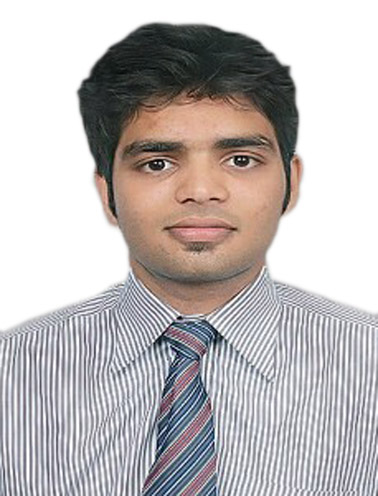
\includegraphics[width=2.5cm, height=3cm]{Photo.jpg}}}}


\newcolumntype{a}{>{\columncolor{Gray}}p}

\begin{document}
\flushleft{

\begin{longtable}{ a{5cm}p{13cm} }
%\hline
%\multicolumn{5}{|c|} \\
%\hline
\newline
\centering{\fcolorbox{blue}{cyan}{\makebox[4.5cm]{\textbf{\uppercase{Objective}}}}}
\flushleft{
The decision about what to put into your paragraphs begins with the germination of a seed of ideas; this "germination process" is better known as brainstorming. There are many techniques for brainstorming; whichever one you choose, this stage of paragraph development cannot be skipped.}\newline

\centering{\fcolorbox{blue}{cyan}{\makebox[4.5cm]{\textbf{\uppercase{skills}}}}}\newline

\begin{itemize}[noitemsep,nolistsep]
	\item AutoCAD, Solidworks, AutoCAD Mechanical, Autodesk Inventor
	\item Excel, C++, HTML, Javascript, Python
	\item Management, Leadership, Organization, Public Speaking, Problem-solving, Teamwork\newline
\end{itemize}


{\fcolorbox{blue}{cyan}{\makebox[4.5cm]{\textbf{\uppercase{Hobbies}}}}}\newline

\begin{itemize}[noitemsep,nolistsep]
	\item Reading Different kinds of books, Programming, listening to classical Indian music
	\item Blogging, Volunteering, Traveling, Art, Design, Music, Reading, Video Gaming.\newline
\end{itemize}



{\fcolorbox{blue}{cyan}{\makebox[4.5cm]{\textbf{\uppercase{Achievements}}}}}\newline

\begin{itemize}[noitemsep,nolistsep]
	\item Was a part of State level football team
	\item Won many national and international level olympiads
	\item having a soft corner towards art\newline
\end{itemize}

&
\newline
{\large{\textbf{\uppercase{Education}}}}\newline

\textbf{Veermata Jijabai Technological Institute (VJTI) } \newline \textbf{From} 14/08/2019 \textbf{To} 14/08/2023 \hspace{1cm} \textbf{CGPA} 10 \hspace{1cm}  \textbf{Percentage} - \newline \textbf{Core Classes}
Thermodynamics, Fluid Mechanics, Coding, Mechatronics, Entreprenuership \newline
\textbf{Professional Associations} 
\begin{itemize}[noitemsep,nolistsep]
	\item Member of Entrepreneurship-cell VJTI
    \item Member of American Society of Mechanical Engineers(ASME)(VJTI)
    \item Member of Institute of Electrical and Electronics Engineers(IEEE)(VJTI)\newline
\end{itemize} 


\textbf{South Indian Education Society(SIES)} \newline \textbf{From} 15/06/2017 \textbf{To} 20/03/2019 \hspace{1cm}  \textbf{CGPA} -  \hspace{1cm}      \textbf{Percentage} 91\% \newline \textbf{Core Classes}
Studied For JEE Mains and Advanced and various other competitive exams \newline
\textbf{Professional Associations} 
\begin{itemize}[noitemsep,nolistsep]
	\item Member of Entrepreneurship-cell VJTI
    \item Member of American Society of Mechanical Engineers(ASME)(VJTI)
    \item Member of Institute of Electrical and Electronics Engineers(IEEE)(VJTI)\newline
\end{itemize} 

\textbf{South Indian Education Society(SIES)} \newline \textbf{From} 15/06/2017 \textbf{To} 20/03/2019 \hspace{1cm}  \textbf{CGPA} -  \hspace{1cm}  \textbf{Percentage} 91\% \newline \textbf{Core Classes}
Studied For JEE Mains and Advanced and various other competitive exams \newline
\textbf{Professional Associations} 
\begin{itemize}[noitemsep,nolistsep]
	\item Member of Entrepreneurship-cell VJTI
    \item Member of American Society of Mechanical Engineers(ASME)(VJTI)
    \item Member of Institute of Electrical and Electronics Engineers(IEEE)(VJTI)\newline
\end{itemize} 


{\large{\textbf{\uppercase{Projects}}}}\newline

\begin{enumerate}[noitemsep,nolistsep]
	\item {\textbf{Resume Builder}}\hfill {\textbf{From}}: May-20 {\textbf{To}} July-20\newline
	Piranhas rarely feed on large animals; they eat smaller fish and aquatic plants. When confronted with humans, piranhas' first instinct is to flee, not attack. 
	\item {\textbf{Fan Controlled using Bluetooth}}\hfill {\textbf{From}}: Dec-19 {\textbf{To}} Mar-20\newline
	Although most people consider piranhas to be quite dangerous, they are, for the most part, entirely harmless. Piranhas rarely feed on large animals;
	\item {\textbf{Fan Controlled using Bluetooth}}\hfill {\textbf{From}}: Dec-19 {\textbf{To}} Mar-20\newline
	Although most people consider piranhas to be quite dangerous, they are, for the most part, entirely harmless. Piranhas rarely feed on large animals; \newline
\end{enumerate}


{\large{\textbf{\uppercase{Internships}}}}\newline

\begin{enumerate}[noitemsep,nolistsep]
	\item {\textbf{Internship at Google}}\hfill {\textbf{From}}: Mar-20 {\textbf{To}} May-20\newline
	Developing writers can often benefit from examining an essay, a paragraph, or even a sentence to determine what makes it effective.
	\item {\textbf{Internship at Lockheed Martin}}\hfill {\textbf{From}}: May-20 {\textbf{To}} Nov-20\newline
	 Scientists' research has revealed that viruses are by far the most abundant life forms on Earth. 
	 \item {\textbf{Internship at Lockheed Martin}}\hfill {\textbf{From}}: May-20 {\textbf{To}} Nov-20\newline
	 Scientists' research has revealed that viruses are by far the most abundant life forms on Earth.
	 
\end{enumerate}


%\hline
\end{longtable} }
\end{document}
